\documentclass[border=10pt]{standalone}

\usepackage{tikz}
\usepackage{tikzsymbols}
\usetikzlibrary{calc,patterns,shapes.geometric}

\def\centerarc[#1](#2)(#3:#4:#5){\draw[#1] ($(#2)+({#5*cos(#3)},{#5*sin(#3)})$) arc (#3:#4:#5);}

\begin{document}
	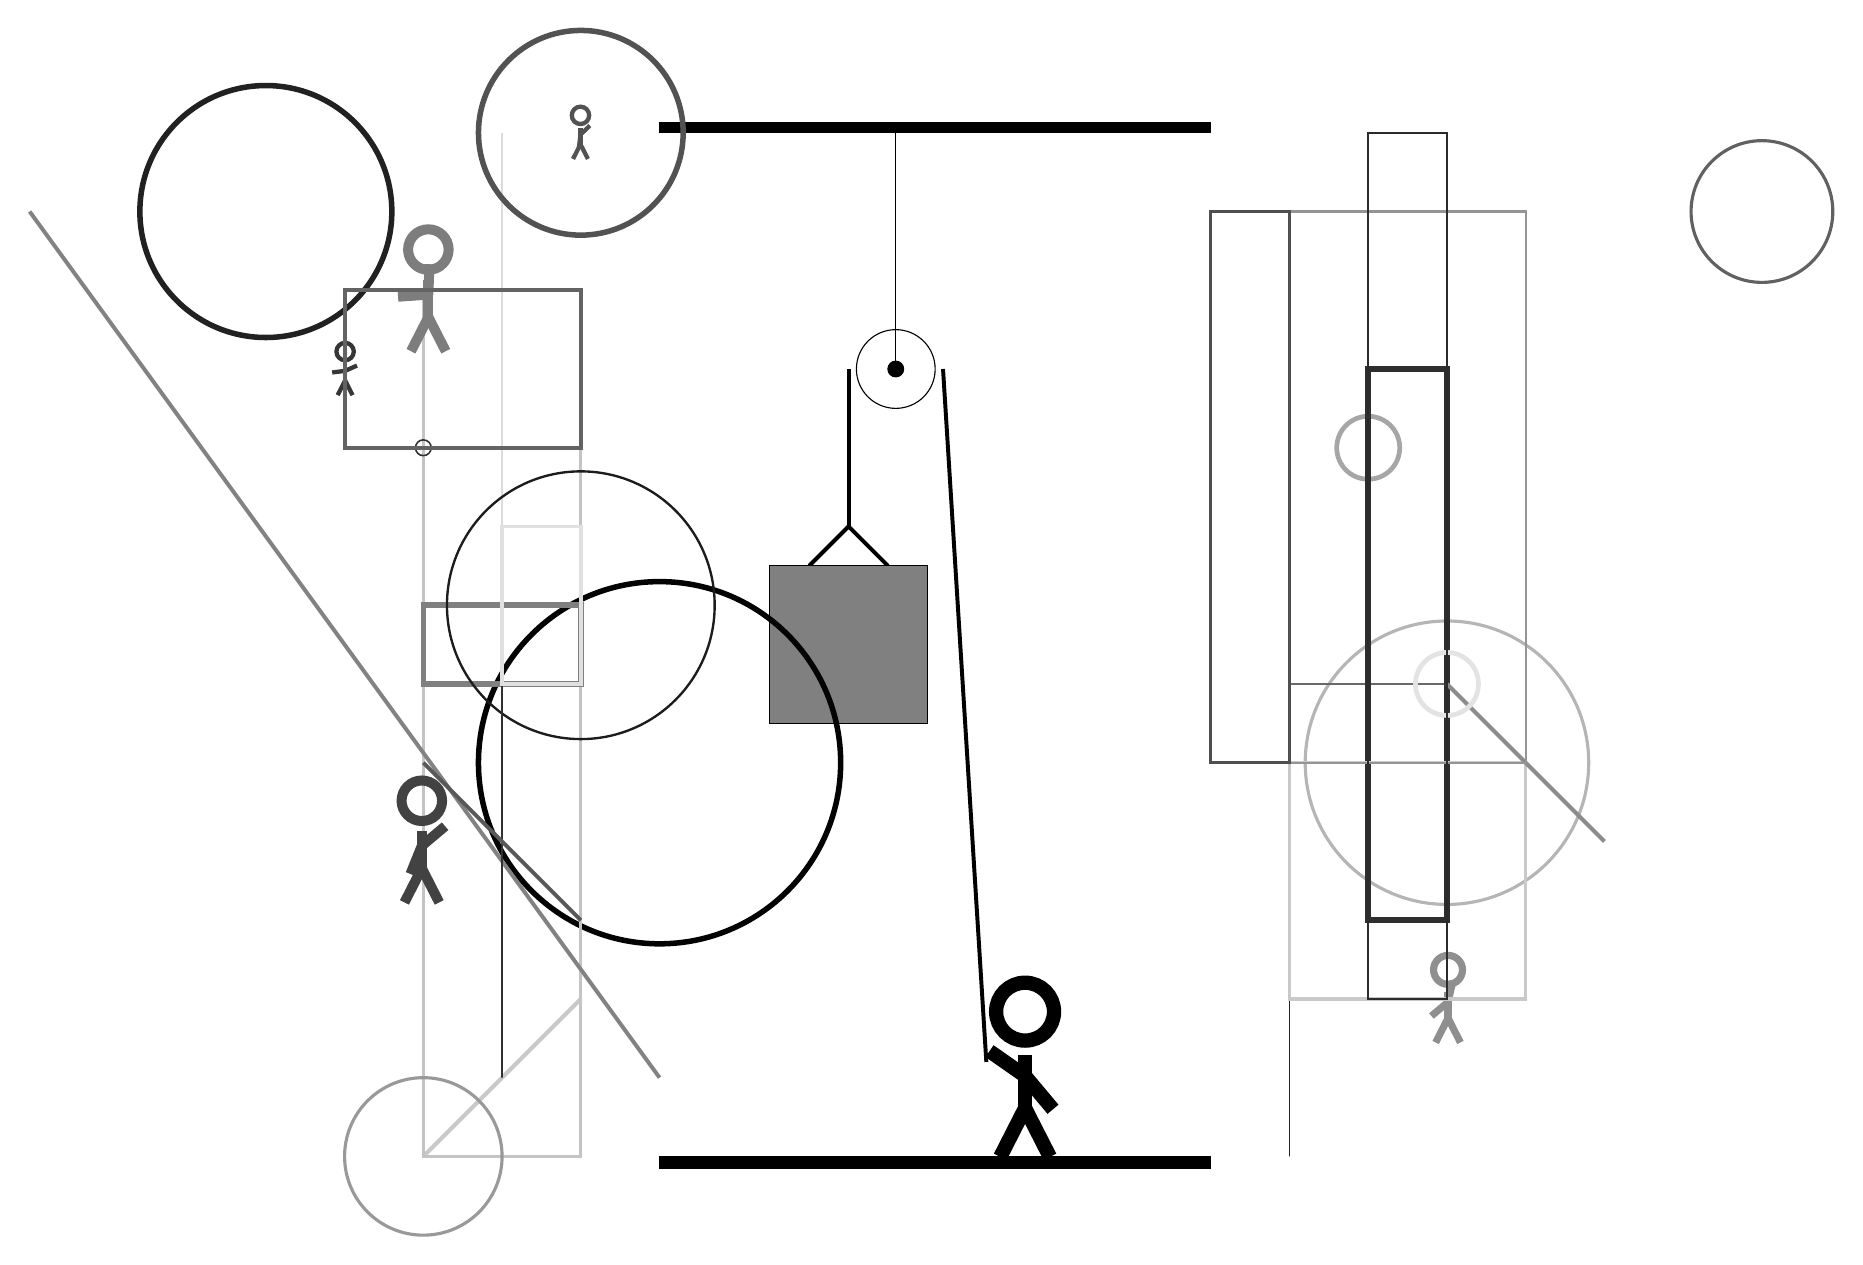
\begin{tikzpicture}
		%%%%% START %%%%%
		
		\draw[fill=black] (-2, 10) rectangle (5, 10.125);
		
		\draw (1, 7) circle (0.5);
		\draw[fill=black] (1, 7) circle (0.1);
		\draw (1, 10) -- (1, 7);
		
		\draw[line width=0.5mm] (-0.1, 4.5) -- (0.4, 5.0) -- (0.9, 4.5);
		\draw[fill=black!50] (-0.6, 4.5) rectangle (1.4, 2.5);
		
		\draw[line width=0.5mm] (0.4, 7) -- (0.4, 5.0);
		\centerarc[line width=0.5mm](1, 7)(0:180:0.6);
		\draw[line width=0.5mm](1.6, 7) -- (2.15, -1.8);
		
		\node at (2.6, -1.9) {\Strichmaxerl[10][-35][-50]};
		
		\draw [line width=0.4mm, color=black!29](8, 2) circle (1.8);
		
		\draw[line width=0.2mm, color=black!14] (-4, 5) rectangle (-4, 10);
		\draw [line width=0.4mm, color=black!62](12, 9) circle (0.9);
		\draw[line width=0.2mm, color=black!87] (6, -3) rectangle (6, 4);
		\node[line width=0.5mm, color=black!44] at (8, -1) {\Strichmaxerl[5][40][77]};
		\draw[line width=0.3mm, color=black!59] (6, -1) rectangle (8, 3);
		\draw [line width=0.7mm, color=black!87](-7, 9) circle (1.6);
		\draw [line width=0.7mm, color=black!99](-2, 2) circle (2.3);
		\draw[line width=0.5mm, color=black!21](-3, -1) -- (-5, -3);
		\node[line width=0.6mm, color=black!79] at (-6, 7) {\Strichmaxerl[3][7][24]};
		
		\draw [line width=0.6mm, color=black!35](7, 6) circle (0.4);
		\draw [line width=0.7mm, color=black!68](-3, 10) circle (1.3);
		\draw[line width=0.4mm, color=black!23] (-3, 8) rectangle (-5, -3);
		
		\draw [line width=0.4mm, color=black!40](-5, -3) circle (1.0);
		\draw[line width=0.5mm, color=black!49](-2, -2) -- (-10, 9);
		\node[line width=0.2mm, color=black!68] at (-3, 10) {\Strichmaxerl[3][83][44]};
		
		\draw[line width=0.7mm, color=black!50] (-3, 3) rectangle (-5, 4);
		\node[line width=0.4mm, color=black!74] at (-5, 1) {\Strichmaxerl[7][68][40]};
		\node[line width=0.7mm, color=black!51] at (-5, 8) {\Strichmaxerl[7][4][88]};
		\draw[line width=0.7mm, color=black!82] (7, 7) rectangle (8, 0);
		\draw[line width=0.4mm, color=black!21] (6, 2) rectangle (9, -1);
		
		\draw[line width=0.5mm, color=black!45](10, 1) -- (8, 3);
		\draw [line width=0.2mm, color=black!81](-5, 6) circle (0.1);
		\draw[line width=0.5mm, color=black!61] (-3, 6) rectangle (-6, 8);
		\draw[line width=0.3mm, color=black!42] (6, 2) rectangle (9, 9);
		
		\draw [line width=0.3mm, color=black!89](-3, 4) circle (1.7);
		
		\draw[line width=0.4mm, color=black!69] (6, 2) rectangle (5, 9);
		\draw[line width=0.3mm, color=black!81] (-4, -2) rectangle (-4, 5);
		\draw[line width=0.5mm, color=black!12] (-4, 3) rectangle (-3, 5);
		\draw [line width=0.6mm, color=black!11](8, 3) circle (0.4);
		\draw[line width=0.3mm, color=black!83] (7, 10) rectangle (8, -1);
		
		\draw[line width=0.5mm, color=black!65](-5, 2) -- (-3, 0);
		
		\draw[fill=black] (-2, -3) rectangle (5, -3.15);
		
		%%%%% END %%%%%
	\end{tikzpicture}
\end{document}